%\setcounter{secnumdepth}{-1}
    \chapter{Multigrid Method}
    \section{Introduction}
    Multigrid (MG) methods in numerical analysis are algorithms for solving differential equations using a hierarchy of discretizations. They are an example of a class of techniques called multiresolution methods, very useful in problems exhibiting multiple scales of behavior.\\
     The main idea of multigrid is to accelerate the convergence of a basic iterative method (known as relaxation, which generally reduces short-wavelength error) by a global correction of the fine grid solution approximation from time to time, accomplished by solving a coarse problem. From \ref{txt:multigrid}
     
%     \subsubsection{Solution Methods} 
%To solve the systems of linear equations we are using this methods:\\
%• Direct\\
%– Gaussian elimination \\
%• Iterative\\
%– Jacobi\\

\section{Multigrid pseudo-code}

The main structure of a MultiGrid algorithm should be describe by following sequence of operations \ref{eq:main}

\begin{align}
	v^h = MultiGrid(A^h, v^h,f^h,\alpha_1, \alpha_2)
	\label{eq:main} 
\end{align}
\begin{equation}
	Relex\quad \alpha_1 \quad times\quad on\quad A^h u^h = f^h \quad on \quad  \Omega^h \quad with \quad arbitrary \quad initial \quad guess \quad v^h
	\label{eq:relax}
\end{equation}
\begin{equation}
\label{eq:computeB}
	compute \quad residual \quad on \quad  fine \quad  grid \quad r^h = f^h - A^hv^h
\end{equation}
\begin{equation}
\label{eq:computeB2h}
	reduce \quad residual \quad on \quad  coarse \quad  grid \quad r^{2h} = I^{2h}_h r^h
\end{equation}
\begin{equation}
	reduce \quad matrix \quad on \quad  coarse \quad  grid \quad A^{2h} = I^{h}_{2h} A^h I_{h}^{2h}
\end{equation}
\begin{equation}
\label{eq:recursivecall}
	Recursive\quad call\quad to\quad MultiGrid \  to \  solve \quad A^{2h}e^{2h} = r^{2h} \quad on \quad \Omega^{2h}
\end{equation}
\begin{equation}
\label{eq:addx}
	correct \quad fine \quad grid \quad solution \quad v^h = v^h + I_{2h}^he^{2h}
\end{equation}
\begin{equation}
	Relex\quad \alpha_2 \quad times\quad on\quad A^h u^h = f^h \quad on \quad  \Omega^h \quad with \quad v^h
\end{equation}

In this procedure, we relax  $\alpha_1$ times the system of equation $A^h u^h = f^h$ with the given initial guess $v^h$. In this project we use the Jacobi method. We  compute the residuals $r^h$ with the new $v^h$. After that, we  use the reduction operator on $r^h$. We  reduce the matrix $A^h$ by applying the reduction and interpolation operators. Which return $A^{2h}$. Now, We use the recusrion with our new system $A^{2h}e^{2h} = r^{2h}$ to solve system on coarse grid $\Omega^{2h}$. And after that we correct the solution on fine grid $v^h$ by using the correction $e^{2h}$. And finally, we relax with $\alpha_2$ times our $A^h u^h = f^h$ with the initial guess $v^h$.
\section{Multigrid mehtod Dense matrix}

\subsection{Introduction}

In the multi-grid method, We use the Gauss elimination method as exact solver, Jacobi method for relaxation. Some specific functions for matrix interpolation, matrix reduction, vector interpolation. The main idea is \\
\begin{lstlisting}[language=C, caption=multigrid method idea]
	multi-grid method(a, b, x, recursion)
		if (recursion == 0)
			gauss-elimination method(a, b, x)
			return 
		jacobi method(a, b, x, 10)
		
		\\reduction of vector b
		b2h = Reduction (b - a*x)
		
		\\ initialize 
		x2h = 0
		
		\\ compute a2h, R = reduction matrix, I = interpolation matrix
		a2h = R *  a * I
		
		multi-grid method(a2h, b2h, x2h, recursion-1)
		
		xh = interpolation x2h
		
		x = x + xh
		
		jacobi method(a, b, x, 10)
		
\end{lstlisting}
 
With the reduction, We decrease the size of the vector. For example if we have a vector of size n, after reduction we obtain a new vector of size n/2. We call the multi-grid method again with the reduced  $A$, $b$ and $x$. And we repeat this process until the recursion counter is equal to 0; and when it is 0, It calls the Gauss elimination method to solve the given system by stopping the recursive calls.
 

\subsection{C++ implementation}

The C++ implementation as below:\\
\begin{lstlisting}[language=C, caption=Multigrid method in C++]
	if (recursion == 0) {

        Gauss_elmination_cpu(a, b, x, row);
        return ;
    }
    float *x_new2 = new float[row];

    init_zero(x_new2, row);
    jacobi_method_cpu(a, x, b, x_new2, row, alpha);

    float *b2h = new float[row / 2];
    float *res1 = new float[row];
    float *x_new2h = new float[row];
    float *a2h = new float[(row / 2) * (row / 2)];

    init_zero(b2h, row / 2);
    init_zero(res1, row);
    init_zero(x_new2h, row);
    init_zero(a2h, (row / 2) * (row / 2));

    matrix_x_vector(row, row, x, a, x_new2h);

    add_sub_vector(b, x_new2h, res1, row,  -1);

    reduction_vector(res1, (row / 2), b2h);

    init_zero(x_new2h, row);

    interpolation_reduction_matrix(a, row, a2h);

    if (row / 2 <= 0) {
        cout << "error" << endl;
        return;
    }
    multigrid_method(a2h, x_new2h, b2h, recursion - 1, row / 2, alpha);

    float * res_int = new float[(row * 2) + 1];
    init_zero(res_int, (row * 2) + 1);

    reduction_interpolation_vector(x_new2h, row, res_int);
    add_sub_vector(x, res_int, x, row,  1);

    jacobi_method_cpu(a, x, b, x_new2, row, alpha);
\end{lstlisting}

In CPU, It is the same implementation as I describe above. Firstly, We check if the recursion is
0 or not. If yes, we call the Gauss elimination method and stop the recursion. If not,
We call to Jacobi method alpha times. We calculate the $b_h^{2h}$,$x_h^{2h}$  and $a_h^{2h}$. Size of $x_h^{2h}$ is half of size $x_{2h}^h$. And we call multigrid method recusively with the $b_h^{2h}$,$x_h^{2h}$  and $a_h^{2h}$. And subtract 1 from recursion. After recursion call, We convert $x_h^{2h}$ to $x_{2h}^h$ and add in x. In last, We call Jacabi method again alpha time. 


\subsection{OCCA implemintation}
The OCCA implementation as below:\\
\begin{lstlisting}[language=C, caption=multigrid method in OCCA]
	if (recursion == 0) {
        gauss_elmination_call_gpu(row, o_a, o_b, o_x, device);
        return;
    }
    occa::memory o_d, o_b2h, o_x2h, o_a2h, o_res, o_res_result2h;
    // Allocate memory on the device

    o_d  = device.malloc(row * sizeof(float));
    o_b2h  = device.malloc((row / 2) * sizeof(float));
    o_x2h  = device.malloc(row * sizeof(float));
    o_res  = device.malloc(row * sizeof(float));
    o_a2h  = device.malloc((row / 2) * (row / 2) * sizeof(float));
    o_res_result2h  = device.malloc(((row * 2) + 1) * sizeof(float));

    jacobi_method_call_gpu(row, o_a, o_b, o_x, o_d, device, alpha);

    dense_Matrix_Vector_Multiplication_call_gpu(row, o_a, o_x, o_res, device);

    add_sub_call_gpu(row, o_b, o_res, o_res, device, -1);

    relaxation_reduction_vector(row / 2, o_res, o_b2h, device);

    reduction_interpolation_reduction_matrix_call_gpu(row, o_a, o_a2h, device);

    if (row / 2 <= 0) {
        cout << "error" << endl;
        return;
    }

    multigrid_method_gpu(row / 2, o_a2h, o_b2h, o_x2h, device, recursion - 1, alpha);

    relaxation_interpolation_vector_call_gpu(row, o_x2h, o_res_result2h, device);

    add_sub_call_gpu(row, o_x, o_res_result2h, o_x, device, 1);

    jacobi_method_call_gpu(row, o_a, o_b, o_x, o_d, device, alpha);
\end{lstlisting}

It has same idea like CPU implementation, We just make all calculation on OCCA. And we described before Gauss elimination and Jacobi method in OCCA. 

\subsection{OCCA vs CPU}
\begin{center}
	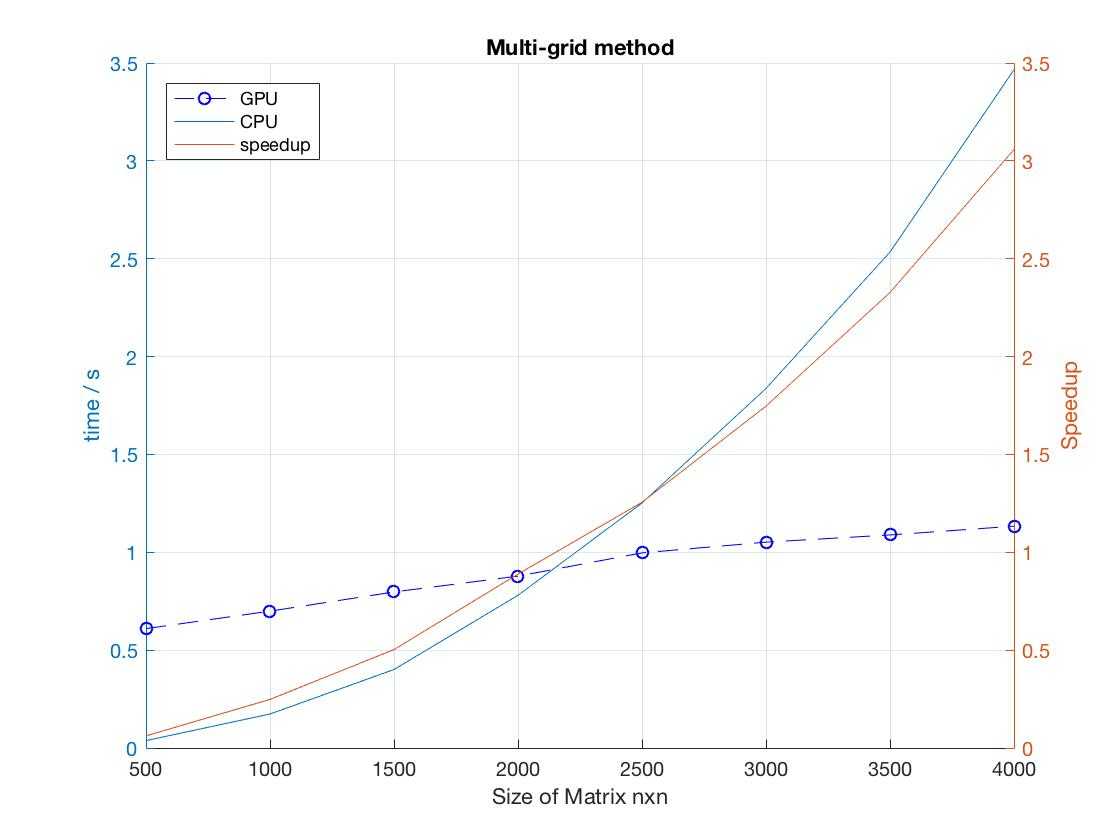
\includegraphics[width = 12cm]{Chapters/multigrid.jpg}
	\captionof{figure}{compare OCCA vs CPU performance}
	\label{img:dmatrix}
\end{center}



In this graph \ref{img:dmatrix} we observe that if the matrix size is small CPU is better than OCCA with GPU. And according to size of matrix, the CPU time increase faster also. But OCCA is increase very slightly. In my opinion, OCCA is much better if the  matrix size is large and OCCA with GPU is faster than CPU. 

\subsection{Numerical analysis of results}
\begin{center}
	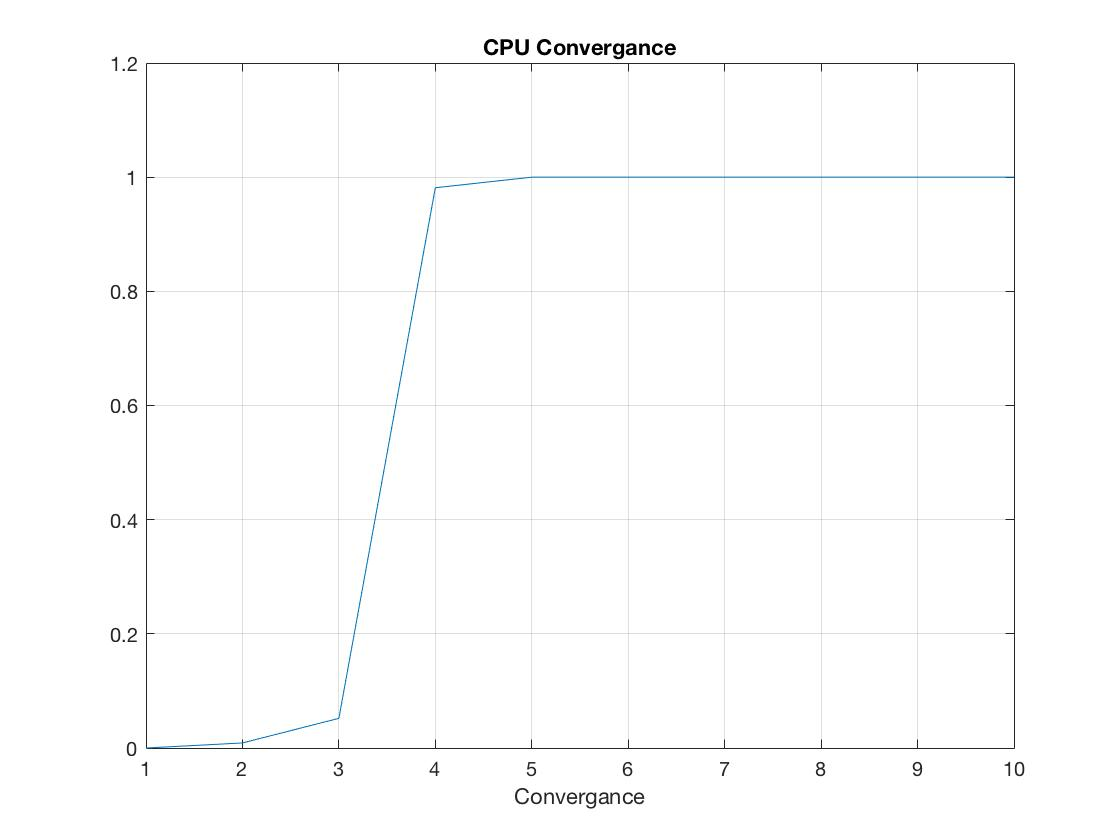
\includegraphics[width = 12cm]{Chapters/cpu_convergence_dense}
	\captionof{figure}{Convergence rate}
	\label{img:convergenceDense}
\end{center}

This convergence rate \ref{img:convergenceDense}, which refer to SPD matrix 2000 by 2000. We have used 32 bit plotting point. In 4s Multigrid step, it converge to solution. 
\section{Multigrid mehtod sparse matrix}
 

\subsection{C++ implementation}

The C++ implementation as below:\\
\begin{lstlisting}[language=C, caption=multigrid method in C++]
	void multigrid_method_sparse_matrix(float a_non_zero[], int a_col_number[], int a_row[], float x[], float b[], int recursion, int row, int alpha, int size_a) {

    if (recursion == 0 || row / 2 < 3 ) {
        int *point = new int[size_a];
        float *aa  = new float [row * row];
        for (int i = 0; i < size_a; i++) {
            point[i] = a_col_number[i] * row + a_row[i];
        }

        vectorToMatrix(row, row, size_a, a_non_zero, aa, point);

        Gauss_elmination_cpu(aa, b, x, row);

        delete [] point;
        delete [] aa;

        return ;
    }


    float *x_new2 = new float[row];
    init_zero(x_new2, row);

    jacobi_method_cpu_sparse_matrix(a_non_zero, a_col_number, a_row, b, x, x_new2, row, alpha, size_a);


    float *b2h = new float[row / 2];
    float *res1 = new float[row];
    float *x_new2h = new float[row];

    init_zero(b2h, row / 2);
    init_zero(res1, row);
    init_zero(x_new2h, row);

    sparse_matrix_x_vector(row, size_a, x, a_row, a_col_number, a_non_zero, x_new2h);
    add_sub_vector(b, x_new2h, res1, row,  -1);
    reduction_vector_sparse(res1, row, b2h);

    init_zero(x_new2h, row);

    int size_non = (size_a + row) * 3;

    float *a2h = new float[size_non];
    int *a2h_row = new int[size_non];
    int *a2h_col = new int[size_non];

    init_zero(a2h, size_non);
    init_zero(a2h_row, size_non);
    init_zero(a2h_col, size_non);


    size_non = interpolation_reduction_matrix_sparse_matrix(a_non_zero, a_col_number, a_row, size_a, row, a2h, a2h_row, a2h_col);

    multigrid_method_sparse_matrix(a2h, a2h_col, a2h_row, x_new2h, b2h, recursion - 1, row / 2, alpha, size_non);

    float * res_int = new float[(row * 2) + 1];

    init_zero(res_int, (row * 2) + 1);

    reduction_interpolation_vector(x_new2h, row, res_int);

    add_sub_vector(x, res_int, x, row,  1);

    init_zero(x_new2, row);

    jacobi_method_cpu_sparse_matrix(a_non_zero, a_col_number, a_row, b, x, x_new2, row, alpha, size_a);


    delete [] x_new2h;
    delete [] b2h;
    delete [] res1;
    delete [] res_int;
    delete [] a2h;
    delete [] a2h_col;
    delete [] a2h_row;
}
\end{lstlisting}

In CPU, It is the same implementation as I describe above. The difference is use of CSR format matrix format rather than use dense matrix with most values 0. Firstly, We check recursion is
0 or not. If yes, we call the Gauss elimination method and stop the recursion. If not,
We call to Jacobi method alpha times. We calculate the $b_h^{2h}$,$x_h^{2h}$  and $a_h^{2h}$. Size of $x_h^{2h}$ is half of size $x_{2h}^h$. And we call multi-grid method recusively with the $b_h^{2h}$,$x_h^{2h}$  and $a_h^{2h}$. And subtract 1 from recursion. After recursion call, We convert $x_h^{2h}$ to $x_{2h}^h$ and add in x. In last, We call jacabi method again alpha time. 


\subsection{OCCA implementation}
The OCCA implementation as below:\\
\begin{lstlisting}[language=C, caption=multigrid method in OCCA]
	void multigrid_method_gpu_sparse_matrix(int row, occa::memory o_a, occa::memory o_a_row, occa::memory o_a_col, occa::memory o_b, occa::memory o_x, occa::device device, int recursion, int alpha, int size_a) {
    if (recursion == 0 || row / 2 <= 3 || size_a < row ) {
        occa::memory o_aa;

        o_aa = device.malloc((row * row) * sizeof(float));

        sparse_vector_to_matrix_gpu_call(row, o_a, o_a_row, o_a_col, device, size_a, o_aa);

        gauss_elmination_call_gpu(row, o_aa, o_b, o_x, device);

        return;
    }

    occa::memory o_b2h, o_x2h, o_a2h, o_a2h_row, o_a2h_col, o_res, o_res2, o_res_result2h, o_row_number ;
    // Allocate memory on the device

    o_b2h  = device.malloc((row / 2) * sizeof(float));
    o_x2h  = device.malloc((row / 2) * sizeof(float));
    o_res  = device.malloc(row * sizeof(float));
    o_res2  = device.malloc(row * sizeof(float));

    int size_non = (size_a + row);
    o_a2h  = device.malloc(size_non * sizeof(float));
    o_a2h_row  = device.malloc(size_non * sizeof(int));
    o_a2h_col  = device.malloc(size_non * sizeof(int));


    jacobi_method_call_gpu_sparse_matrix(row, o_a, o_a_col, o_a_row, o_b, o_x, device,  alpha, size_a);

    sparse_Matrix_Vector_Multiplication_call_gpu(row, size_a, o_a, o_a_row, o_a_col, o_x, o_res, device);

    add_sub_call_gpu(row, o_b, o_res, o_res2, device, -1);

    relaxation_reduction_vector(row / 2, o_res2, o_b2h, device);

    size_non =  reduction_interpolation_reduction_sparse_matrix_call_gpu(row, o_a, o_a_col, o_a_row,  o_a2h, o_a2h_row, o_a2h_col, device, size_a);


    multigrid_method_gpu_sparse_matrix(row / 2, o_a2h, o_a2h_row, o_a2h_col, o_b2h, o_x2h, device, recursion - 1, alpha, size_non);

    o_res_result2h  = device.malloc(((row * 2) + 1) * sizeof(float));

    relaxation_interpolation_vector_call_gpu(row, o_x2h, o_res_result2h, device);

    add_sub_call_gpu(row, o_x, o_res_result2h, o_x, device, 1);

    jacobi_method_call_gpu_sparse_matrix(row, o_a, o_a_col, o_a_row, o_b, o_x, device,  alpha, size_a);
}
\end{lstlisting}

It has same idea like CPU implementation, We just make all calculation on GPU. And we described before Guass elimination and jacobi method in GPU. And, We use the CSR matrix format rather than full matrix size and Gauss elimination method is work only with full matix size. Thats why, We change CSR format matrix to sparse matrix with 0's and than call to Gauss elimination method.

\subsection{OCCA vs CPU}
\begin{center}
	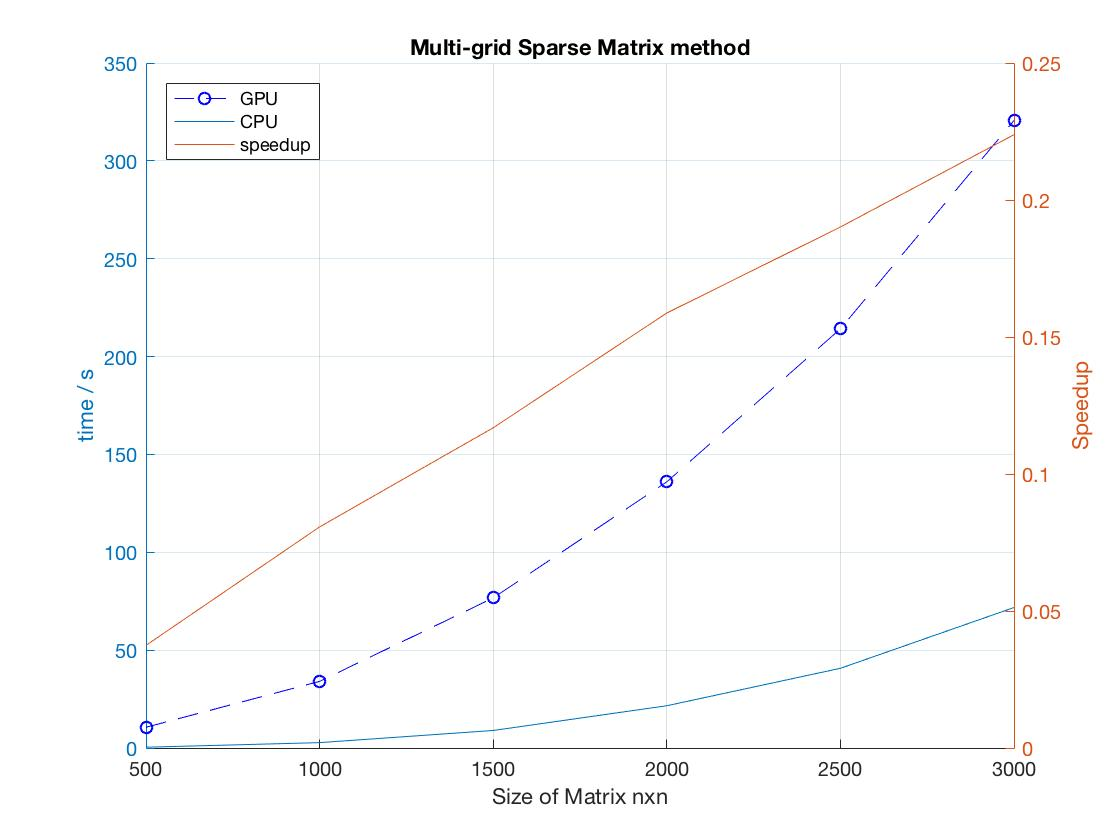
\includegraphics[width = 12cm]{Chapters/multigrid_sparse_matrix.jpg}
	\captionof{figure}{compare OCCA vs CPU performance}
	\label{img:multigridsparse}
\end{center}

%$
%\begin{bmatrix}
%	recursion & size & gputime & cputime & speedup\\
%	8&500&1.97835&0.424889&0.214769\\
%	9&1000&2.30963&2.80448&1.21425\\
%	10&1500&2.7869& 8.92915&3.20398\\
%	10&2000&2.74789&22.0198&8.01333\\
%	11&2500&3.09132&41.114&13.2998\\
%	11&3000&3.2176&68.7087&21.3541\\
%\end{bmatrix}
%$
%
%







%We can see in this graph if matrix size is smaller than 800 than CPU is better than OCCA. And according to size of matrix, the CPU time increase faster also. But OCCA is increase very slightly. In my opinion, OCCA is much better if we have matrix size is bigger than OCCA will be much faster than CPU. 

We can see in this graph \ref{img:multigridsparse} CPU is always faster than OCCA. OCCA, We are call to kernel for each function and copy data also take too much time. We can not implement all the function in kernel, because we do not have any atomic operation in OCCA. We have to return to CPU and call again to kernel. That took too much time. And result, We can see CPU is better than OCCA, but if we consider dense matrix OCCA is better.




\subsection{Numerical analysis of results}
\begin{center}
	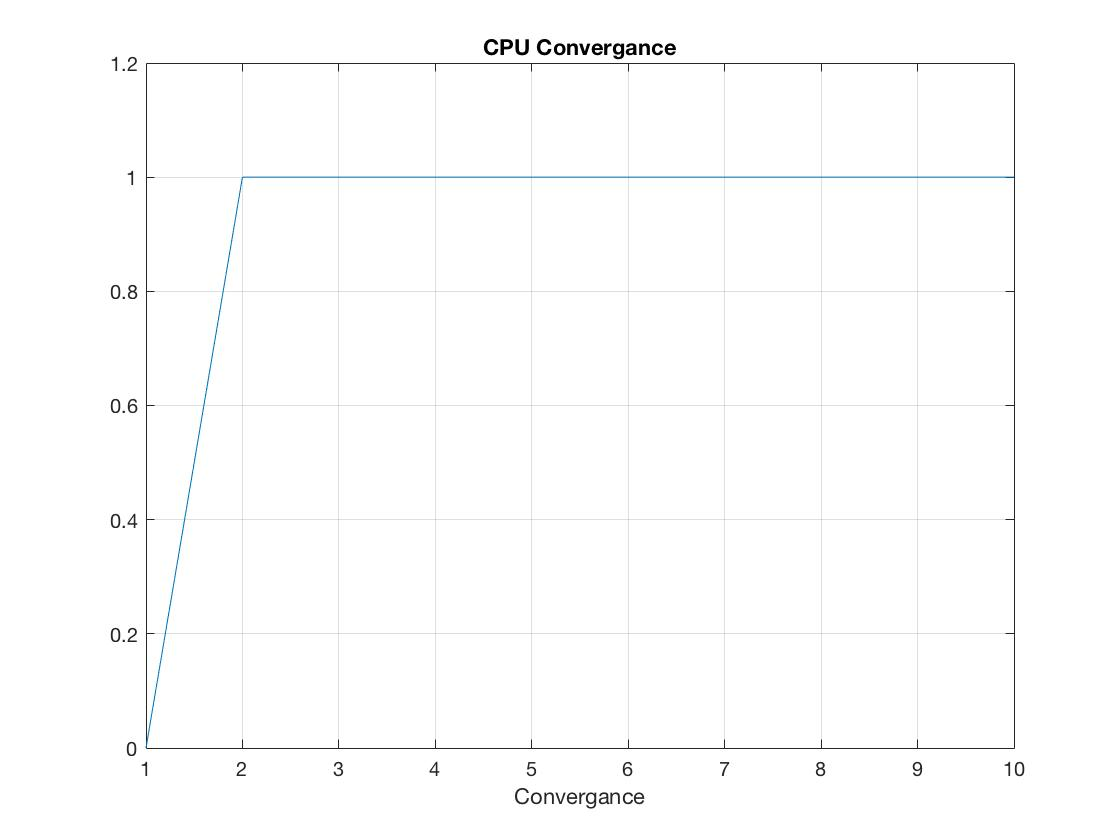
\includegraphics[width = 12cm]{Chapters/cpu_convergence}
	\captionof{figure}{Convergence rate}
	\label{img:convergenceSparse}
\end{center}

This convergence rate \ref{img:convergenceSparse}, which refer to SPD sparse matrix 2000 by 2000 and sparsity ratio is 0.05. We have used 32 bit plotting point. In one Multigrid step, it converge to solution. 













 